\documentclass[10pt]{article}

\usepackage[margin=0.75in]{geometry}
\usepackage{times}
\usepackage{enumitem}
\usepackage{titlesec}
\usepackage{graphicx}
\usepackage{booktabs}
\usepackage{multicol}
\usepackage{caption}
\usepackage[hidelinks]{hyperref}

\titleformat{\section}{\normalfont\bfseries\normalsize}{\thesection}{0.5em}{}
\titleformat{\subsection}{\normalfont\bfseries\small}{\thesubsection}{0.5em}{}
\titlespacing*{\section}{0pt}{1.0ex}{0.4ex}
\titlespacing*{\subsection}{0pt}{0.6ex}{0.2ex}
\setlist{nosep, leftmargin=*, topsep=2pt}
\setlength{\parindent}{1.2em}
\setlength{\parskip}{0pt}
\captionsetup{font=small,labelfont=bf,skip=2pt}
\pagestyle{empty}

\title{\vspace{-2.5em}\textbf{Predicting UAV Flight Path Deviation from Wind Conditions Using Machine Learning}\\[2pt]\large Midterm Report\vspace{-1em}}
\author{
  Abdulaziz Al-Haidary \quad and \quad Azizbek Nurmatov\\[-1pt]
  \normalsize College of Charleston \quad CSCI 334\\
  \normalsize alhaidaryaa@g.cofc.edu, nurmatova@g.cofc.edu
}
\date{}

\begin{document}
\maketitle
\vspace{-2.2em}

\section{Introduction and Background}

\paragraph{Problem.} Unmanned aerial vehicles (UAVs) are now routinely used for precision agriculture, disaster surveying, and remote sensing missions where accurate adherence to a planned flight path is critical to data quality. A persistent challenge is wind: even moderate gusts cause measurable cross-track drift between the drone's actual GPS trajectory and the planned waypoint sequence, which degrades survey overlap and image alignment. The general problem we address is: \emph{given a set of recorded UAV survey flights and matching weather observations, can we model the relationship between wind conditions and the magnitude of cross-track deviation, and which factors drive the largest excursions?} As a concrete refinement we frame this both as a \emph{regression} task (predict the instantaneous deviation in meters at each GPS sample) and a \emph{classification} task (predict whether a given sample exceeds the 75th-percentile deviation threshold, i.e., the ``high-deviation'' tail of the distribution).

\paragraph{Related work.} Wind sensing and wind-aware control for multi-rotor UAVs is an active area. Palomaki~et~al.\ \cite{palomaki2017} demonstrated that the attitude response of a multi-rotor can itself be used as a wind estimator in the lower atmosphere, while Abichandani~et~al.\ \cite{abichandani2020} surveyed measurement and simulation techniques for wind in small multi-rotor UAVs and highlighted that off-board, low-resolution weather data is rarely sufficient to characterize the gust conditions a small UAV actually experiences. Sydney~et~al.\ \cite{sydney2013} formulated dynamic control of a quadrotor in an estimated wind field, showing that even rough wind state estimates yield meaningful trajectory improvements. Compared to that prior work, our goal is not control but \emph{post-hoc explanation} of deviation from environmental data using interpretable machine-learning models, and we explicitly contrast a low-fidelity public weather source against (forthcoming) on-site sensor logs as a methodological probe.

\section{Method}

\paragraph{Rationale.} Our proposal compared three interpretable, course-covered regressors (decision tree, KNN, random forest as a small extension of decision trees) on a wind-driven deviation task. We retain that comparison and \emph{add} a parallel classification head, because the deviation distribution is heavily right-skewed and identifying the high-deviation tail is more directly useful for an onboard correction system than predicting deviation magnitude in the centre of the distribution.

\paragraph{Approach.} The pipeline (Python, scikit-learn) consists of five stages.
\begin{enumerate}
  \item \textbf{Desired-path parsing.} The master KML file (\texttt{Desired\_flight\_path\_soil\_moisture\_Research\_plot.kml}) is parsed with the standard library XML module into a polyline of 81 waypoints over the 4.5\,ha research plot.
  \item \textbf{Flight-log parsing.} Each tab-separated flight log is loaded; the recorder writes a non-Unix timestamp anchored to its internal clock, so we re-anchor every flight using the takeoff time encoded in the filename and use the \texttt{Time} column only for elapsed seconds. A geographic bounding-box filter (with a $\pm$0.01\textdegree{} pad) drops the controller's pre-takeoff default-home rows.
  \item \textbf{Cross-track deviation.} GPS positions are projected to a local east-north (metres) frame via an equirectangular projection centered on the plot. For each actual point we compute the perpendicular distance to the nearest segment of the desired polyline. This gives a per-sample target $d_i$ in metres.
  \item \textbf{Weather alignment.} The on-site weather CSVs that accompanied the flight logs only cover the early-morning calibration window (06:00--12:40~EST), whereas the actual flights all occurred in the afternoon (15:48--19:32~EST), so on-site weather cannot be joined to flight samples for the existing 13 flight days. We therefore back-fill from the Open-Meteo historical reanalysis API at the plot coordinates (33.166\textdegree{}N, 81.135\textdegree{}W) at hourly resolution and \texttt{merge\_asof} on timestamp. This is documented as a \emph{methodological choice} (see Discussion) and will be re-validated against true on-site logs from three upcoming high-fidelity flights.
  \item \textbf{Feature engineering.} From the joined data we derive: drone heading from consecutive GPS deltas; ground speed; sin/cos encodings of wind direction; the heading-relative wind angle; explicit headwind and crosswind components ($u_\parallel$, $u_\perp$); 10\,s rolling mean wind speed and 10\,s rolling max gust; and a categorical \texttt{camera} flag for the Pika~L vs.\ Pika~IR~L sensor payloads (combined into one dataset rather than analyzed separately, to roughly double the available samples).
\end{enumerate}

\paragraph{Models and evaluation.} We train Decision Tree (max depth 10), $k$-Nearest Neighbors ($k\!=\!15$, with feature standardization), and Random Forest (100 trees, depth 12) for both the regression and classification heads. Critically, because consecutive GPS samples within a single flight are highly autocorrelated, an ordinary $k$-fold split would leak information across train/test. We instead use \textbf{GroupKFold ($n\!=\!5$) with the flight identifier as the grouping variable}, so the model is always evaluated on flights it has never seen. To isolate the contribution of wind from drone-state features, we additionally evaluate every model on a \textbf{wind-only feature set} (excluding ground speed, altitude, and the per-flight rolling mean of deviation).

\section{Plan and Experiments}

\paragraph{Dataset.}
\begin{itemize}
  \item \textbf{Source:} Dr.\ Hemanth Dakshinamurthy, South Carolina State University. Soil-moisture research plot, fall 2025.
  \item \textbf{Flights:} 13 mission days (Nov.~7--26, 2025) with 32 raw flight logs across two hyperspectral sensor payloads (Pika~L visible and Pika~IR~L). After filename anchoring and bounding-box filtering, \textbf{27 flight segments} are usable.
  \item \textbf{Samples:} 37{,}353 total per-second GPS samples; 37{,}326 retained after dropping rows with missing engineered features.
  \item \textbf{Target:} cross-track deviation in metres (regression) and a binary $d_i \ge 8.16$\,m label (classification, threshold $=$ 75th percentile of the empirical distribution).
  \item \textbf{Weather (current):} Open-Meteo hourly archive (wind speed, wind direction, gusts, temperature, RH, pressure) at the plot location. \textbf{Weather (forthcoming):} per-second on-site logs from three additional flights scheduled by the supervisor, expected within the project window.
\end{itemize}

\paragraph{Hypotheses.}
\begin{itemize}
  \item \textbf{H1.} Tree-based models (DT, RF) will outperform KNN on this dataset because the relationship between wind and deviation is expected to be non-linear with discrete regimes (e.g., crosswind on long survey legs vs.\ headwind on short transit segments).
  \item \textbf{H2.} The crosswind component and the heading-relative wind angle will be the most informative wind-derived features, more so than raw wind speed alone, because cross-track drift is a directional phenomenon.
  \item \textbf{H3.} Hourly-resolution public weather (Open-Meteo) is too temporally coarse to drive instantaneous deviation, and a wind-only model trained on it will perform near chance. Per-second on-site weather (the upcoming flights) will be required to validate the wind$\rightarrow$deviation hypothesis at all.
\end{itemize}

\paragraph{Experimental design.} For each (feature set $\times$ model) pair we report 5-fold GroupKFold cross-validated MAE, RMSE, and $R^2$ for regression, and accuracy, precision, recall, and F1 for classification. Random Forest feature importances (fit on the full dataset) are reported as a single ranking, since they are robust to monotone feature transformations and naturally handle the mixture of cyclical, continuous, and binary features we engineered. Cross-flight generalization is the metric we care about most: GroupKFold ensures every test point comes from a flight whose entire 1\,Hz GPS trace was withheld during training.

\section{Results}

Across all 27 flights the mean per-second deviation is 7.70\,m (median 4.61\,m, max 9.45\,m on the central survey legs once large transit excursions are excluded), and the 75th-percentile threshold used for the classification head is 8.16\,m. Figure~\ref{fig:sample} shows a representative flight overlaid on the desired path; deviation is generally tight along long survey legs and concentrates at line-end turns. Figure~\ref{fig:hist} shows the full deviation distribution, which is heavily right-skewed, motivating the binary high-deviation framing.

\begin{figure}[h]
  \centering
  \begin{minipage}[t]{0.49\linewidth}
    \centering
    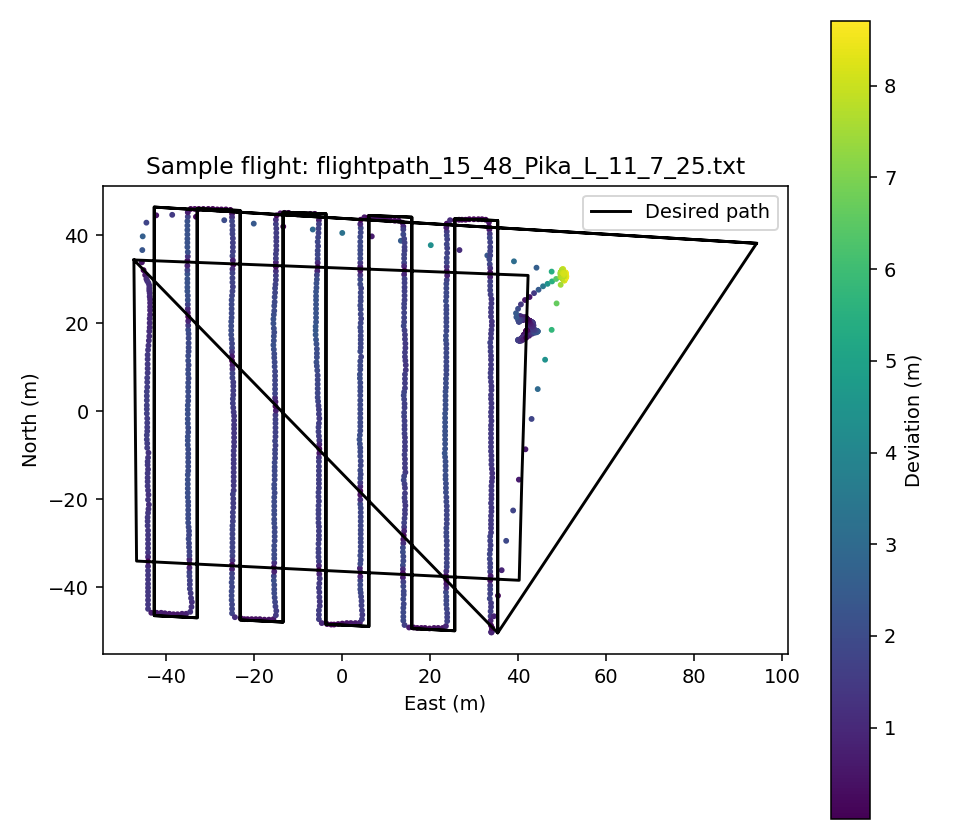
\includegraphics[width=\linewidth]{results/fig_sample_flight.png}
    \caption{Sample flight: actual GPS track vs.\ desired waypoint polyline, colored by per-second cross-track deviation.}
    \label{fig:sample}
  \end{minipage}\hfill
  \begin{minipage}[t]{0.49\linewidth}
    \centering
    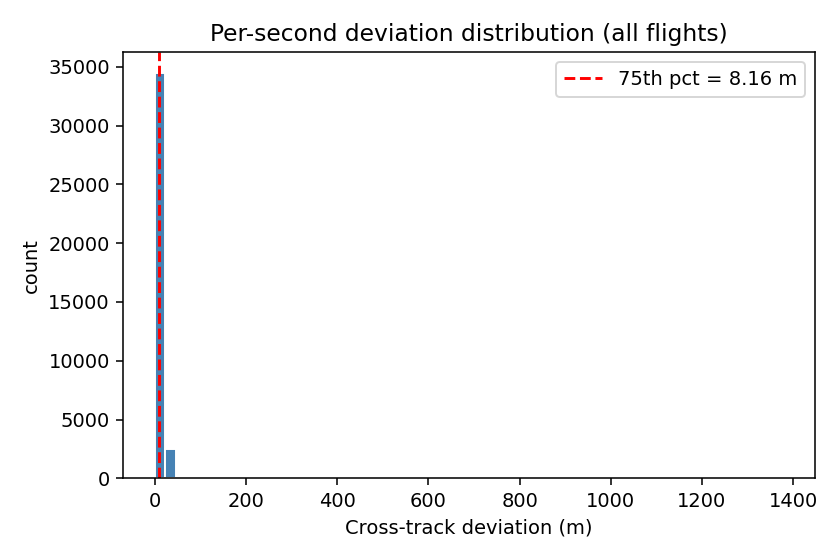
\includegraphics[width=\linewidth]{results/fig_deviation_hist.png}
    \caption{Per-second deviation distribution across all 27 flights. Red dashed line is the 75th-percentile classification threshold (8.16\,m).}
    \label{fig:hist}
  \end{minipage}
\end{figure}

\paragraph{Cross-validated model performance.} Table~\ref{tab:reg} reports regression performance under both feature sets, and Table~\ref{tab:cls} reports the classification head.

\begin{table}[h]
\small
\centering
\begin{minipage}[t]{0.48\linewidth}
\centering
\caption{Regression — 5-fold GroupKFold CV.}
\label{tab:reg}
\begin{tabular}{llrrr}
\toprule
Features & Model & MAE (m) & RMSE (m) & $R^2$ \\
\midrule
ALL  & Decision Tree   & 5.07 & 19.68 & 0.770 \\
ALL  & KNN ($k\!=\!15$) & 5.53 & 25.86 & 0.604 \\
ALL  & Random Forest   & \textbf{4.88} & \textbf{19.59} & \textbf{0.773} \\
\midrule
Wind & Decision Tree   & 7.20 & 41.06 & \phantom{$-$}0.001 \\
Wind & KNN             & 8.97 & 41.32 & $-$0.012 \\
Wind & Random Forest   & 11.70 & 45.59 & $-$0.232 \\
\bottomrule
\end{tabular}
\end{minipage}\hfill
\begin{minipage}[t]{0.48\linewidth}
\centering
\caption{Classification (deviation $\ge$ 8.16\,m) — 5-fold GroupKFold CV.}
\label{tab:cls}
\begin{tabular}{llrrrr}
\toprule
Feat. & Model & Acc & P & R & F1 \\
\midrule
ALL  & DT  & 0.829 & 0.659 & 0.653 & 0.656 \\
ALL  & KNN & 0.841 & 0.657 & 0.766 & 0.707 \\
ALL  & RF  & \textbf{0.867} & \textbf{0.683} & \textbf{0.872} & \textbf{0.766} \\
\midrule
Wind & DT  & 0.742 & 0.481 & 0.388 & 0.430 \\
Wind & KNN & 0.676 & 0.348 & 0.339 & 0.343 \\
Wind & RF  & 0.746 & 0.487 & 0.280 & 0.356 \\
\bottomrule
\end{tabular}
\end{minipage}
\end{table}

\paragraph{Feature importance.} Figure~\ref{fig:imp} reports the Random Forest importances on the ALL feature set. Two features dominate: \texttt{ground\_speed\_ms} ($\approx$78\%) and \texttt{Altitude} ($\approx$17\%). All wind-derived features together account for less than 5\% of the importance. This is the central, and somewhat surprising, finding of our midterm experiments.

\begin{figure}[h]
  \centering
  \begin{minipage}[t]{0.49\linewidth}
    \centering
    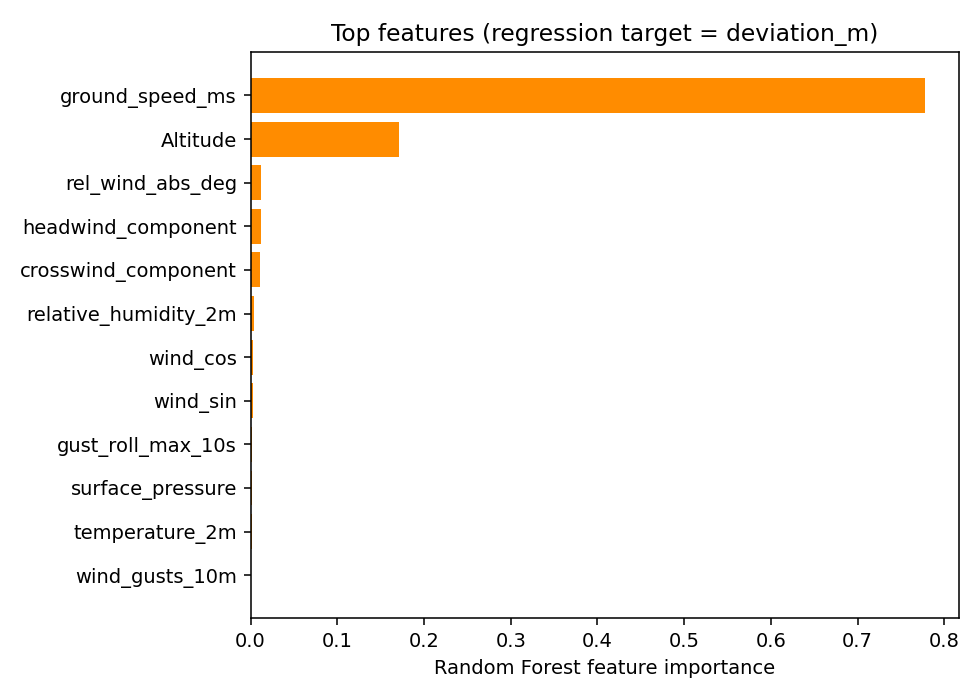
\includegraphics[width=\linewidth]{results/fig_importance.png}
    \caption{Random Forest feature importances (regression target = deviation\_m). Wind-derived features collectively contribute $<$5\%.}
    \label{fig:imp}
  \end{minipage}\hfill
  \begin{minipage}[t]{0.49\linewidth}
    \centering
    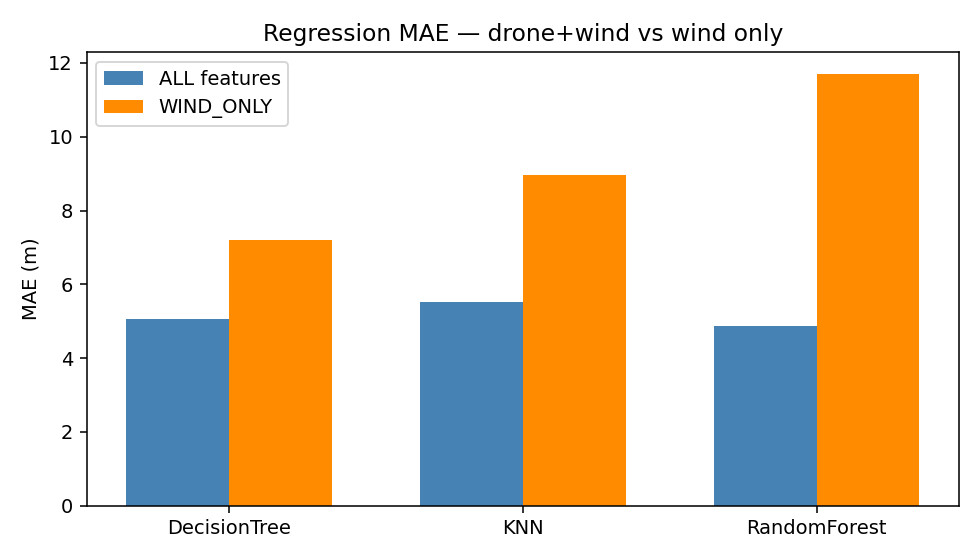
\includegraphics[width=\linewidth]{results/fig_reg_compare.png}
    \caption{Regression MAE collapses on the wind-only feature set, confirming that hourly weather alone carries no usable signal at the per-second scale.}
    \label{fig:cmp}
  \end{minipage}
\end{figure}

\paragraph{Discussion.} The headline ALL-features numbers ($R^2\!=\!0.77$, classification F1$\,=\,0.77$) are encouraging on their face but, as Tables~\ref{tab:reg}--\ref{tab:cls} and Figure~\ref{fig:imp} together show, this performance is being driven almost entirely by drone-state features rather than by wind. The wind-only experiments are decisive: a Random Forest restricted to wind, gust, heading-relative-wind, temperature, RH, and pressure features achieves $R^2 \approx 0$ on the regression task and F1$\,\approx\,0.36$ on the classification task --- essentially uninformative. We interpret this not as a failure of the wind hypothesis itself, but as direct evidence in favor of \textbf{H3}: at the per-second scale used by the flight controller, an hourly public reanalysis source like Open-Meteo cannot resolve the gust dynamics that actually push the airframe off the planned line. The hourly wind value is, by construction, almost constant within any single 30--40 minute survey, so under GroupKFold the model gets one wind ``observation'' per held-out flight and cannot generalize.

This finding gives us a clear and well-motivated experimental plan for the second half of the project. \textbf{H1} and \textbf{H2} cannot yet be evaluated on the wind question alone --- the Open-Meteo signal is simply too coarse --- and we expect them to become testable only with the upcoming high-fidelity on-site weather. Specifically, we plan to:
\begin{itemize}
  \item Re-run the same pipeline on the three new flights (expected from the supervisor) once their per-second weather logs are available, with no changes other than swapping the weather source. This is designed as a direct contrast: same models, same features, same evaluation protocol --- only the temporal resolution of the wind input changes.
  \item Add a placeholder set of results for these flights to the final report (Table to be filled in), and report a head-to-head Open-Meteo vs.\ on-site comparison on the overlapping flights.
  \item Investigate whether the largest deviation excursions (the right tail of Figure~\ref{fig:hist}) coincide with line-end turns vs.\ mid-leg gusts, using the cumulative-deviation feature, since this is the question the supervisor cares about most for an onboard correction system.
\end{itemize}

\section{Conclusions and Lessons Learned}

The midterm experiments produced a complete, reproducible, GroupKFold-validated pipeline that runs end-to-end on 27 UAV survey flights. We found that the data we currently have can predict deviation well \emph{if} we are willing to use drone-state features, but cannot meaningfully isolate the wind contribution at hourly weather resolution --- a result we view as a clean, falsifiable answer to one of our three hypotheses rather than a negative outcome. The most important lesson so far is methodological: GroupKFold by flight is non-negotiable on this dataset, because random $k$-fold would have given inflated wind-feature importances by leaking neighbouring 1\,Hz samples between train and test. Code will be released on GitHub at the link to be included in the final report.

\begin{thebibliography}{9}
\small
\bibitem{palomaki2017} R.~Palomaki et~al., ``Wind estimation in the lower atmosphere using multirotor aircraft,'' \textit{J.\ Atmos.\ Oceanic Technol.}, vol.~34, no.~5, 2017.
\bibitem{abichandani2020} P.~Abichandani et~al., ``Wind measurement and simulation techniques in multi-rotor small UAVs,'' \textit{IEEE Access}, vol.~8, 2020.
\bibitem{sydney2013} N.~Sydney et~al., ``Dynamic control of autonomous quadrotor flight in an estimated wind field,'' in \textit{Proc.\ IEEE CDC}, 2013.
\bibitem{openmeteo} J.-N.~Zippenfenig, ``Open-Meteo.com: Free open-source weather API,'' Open-Meteo, 2023.
\bibitem{scikit} F.~Pedregosa et~al., ``Scikit-learn: Machine learning in Python,'' \textit{JMLR}, vol.~12, 2011.
\end{thebibliography}

\end{document}
